%%%%%%%%%%%%%%%%%%% vorlage.tex %%%%%%%%%%%%%%%%%%%%%%%%%%%%%
%
% LaTeX-Vorlage zur Erstellung von Projekt-Dokumentationen
% im Fachbereich Informatik der Hochschule Trier
%
% Basis: Vorlage svmono des Springer Verlags
%
%%%%%%%%%%%%%%%%%%%%%%%%%%%%%%%%%%%%%%%%%%%%%%%%%%%%%%%%%%%%%

\documentclass[envcountsame,envcountchap, deutsch]{i-studis}

\usepackage{makeidx}         	% Index
\usepackage{multicol}        	% Zweispaltiger Index
%\usepackage[bottom]{footmisc}	% Erzeugung von Fu�noten

%%-----------------------------------------------------
%\newif\ifpdf
%\ifx\pdfoutput\undefined
%\pdffalse
%\else
%\pdfoutput=1
%\pdftrue
%\fi
%%--------------------------------------------------------
%\ifpdf
\usepackage[pdftex]{graphicx}
\usepackage{epstopdf}
\usepackage[pdftex,plainpages=false]{hyperref}
%\else
%\usepackage{graphicx}
%\usepackage[plainpages=false]{hyperref}
%\fi

%%-----------------------------------------------------
\usepackage{color}				% Farbverwaltung
%\usepackage{ngerman} 			% Neue deutsche Rechtsschreibung
\usepackage[english, ngerman]{babel}
\usepackage[latin1]{inputenc} 	% Erm�glicht Umlaute-Darstellung
%\usepackage[utf8]{inputenc}  	% Erm�glicht Umlaute-Darstellung unter Linux (je nach verwendetem Format)

%-----------------------------------------------------
\usepackage{listings} 			% Code-Darstellung
\lstset
{
	basicstyle=\scriptsize, 	% print whole listing small
	keywordstyle=\color{blue}\bfseries,
								% underlined bold black keywords
	identifierstyle=, 			% nothing happens
	commentstyle=\color{red}, 	% white comments
	stringstyle=\ttfamily, 		% typewriter type for strings
	showstringspaces=false, 	% no special string spaces
	framexleftmargin=7mm, 
	tabsize=3,
	showtabs=false,
	frame=single, 
	rulesepcolor=\color{blue},
	numbers=left,
	linewidth=146mm,
	xleftmargin=8mm
}
\usepackage{textcomp} 			% Celsius-Darstellung
\usepackage{amssymb,amsfonts,amstext,amsmath}	% Mathematische Symbole
\usepackage[german, ruled, vlined]{algorithm2e}
\usepackage[a4paper]{geometry} % Andere Formatierung
\usepackage{bibgerm}
\usepackage{array}
\hyphenation{Ele-men-tar-ob-jek-te  ab-ge-tas-tet Aus-wer-tung House-holder-Matrix Le-ast-Squa-res-Al-go-ri-th-men} 		% Weitere Silbentrennung bei Bedarf angeben
\setlength{\textheight}{1.1\textheight}
\pagestyle{myheadings} 			% Erzeugt selbstdefinierte Kopfzeile
\makeindex 						% Index-Erstellung


%--------------------------------------------------------------------------
\begin{document}
%------------------------- Titelblatt -------------------------------------
\title{Titel der Arbeit}
\project{Ausarbeitung zur Vorlesung Wissenschaftliches Arbeiten}
%--------------------------------------------------------------------------
\supervisor{Prof. Dr. J�rg Lohscheller} 		% Betreuer der Arbeit
\author{Bearbeiter 1: Bernardo Jose Barcia Cordero \\Bearbeiter 2: Simon Deutscher \\Bearbeiter 3: Felix Kalchschmid}							% Autor der Arbeit
\groupid{183}
\address{Trier,} 							% Im Zusammenhang mit dem Datum wird hinter dem Ort ein Komma angegeben
\submitdate{21.06.2020} 				% Abgabedatum
%\begingroup
%  \renewcommand{\thepage}{title}
%  \mytitlepage
%  \newpage
%\endgroup
\begingroup
  \renewcommand{\thepage}{Titel}
  \mytitlepage
  \newpage
\endgroup
%--------------------------------------------------------------------------
\frontmatter 
%--------------------------------------------------------------------------
\kurzfassung

%% deutsch
\paragraph*{}
%In der Kurzfassung soll in kurzer und pr"agnanter Weise der wesentliche Inhalt der Arbeit beschrieben werden. Dazu z"ahlen vor allem eine kurze Aufgabenbeschreibung, der L�sungsansatz sowie die wesentlichen Ergebnisse der Arbeit. Ein h"aufiger Fehler f"ur die Kurzfassung ist, dass lediglich die Aufgabenbeschreibung (d.h. das Problem) in Kurzform vorgelegt wird. Die Kurzfassung soll aber die gesamte Arbeit widerspiegeln. Deshalb sind vor allem die erzielten Ergebnisse darzustellen. Die Kurzfassung soll etwa eine halbe bis ganze DIN-A4-Seite umfassen.
%\newline
%Hinweis: Schreiben Sie die Kurzfassung am Ende der Arbeit, denn eventuell ist Ihnen beim Schreiben erst vollends klar geworden, was das Wesentliche der Arbeit ist bzw. welche Schwerpunkte Sie bei der Arbeit gesetzt haben. Andernfalls laufen Sie Gefahr, dass die Kurzfassung nicht zum Rest der Arbeit passt.

Die vorliegende Arbeit nimmt sich zum Ziel die Funktionsprinzipien und Anwendungen der Pfadplanung zu erl"autern. Dazu wird die anf"anglich die Vorgehensweise bei der Pfadplanung beschrieben und die wichtigsten Grundlagen erkl"art. Die Algorithmen werden am Beispiel der Pfadplanung im diskreten Zustandsraum eingef�hrt und auf die Unterschiede eingegangen. Der kontinuierliche Zustandsraum wird hingegen bei den Anwendungen erl�utert und durch Anwendungsbeispiele veranschaulicht.
Es wird dadurch ein Grundverst"andis erreicht, um im folgenden selbst entscheiden zu k"onnen, in welches Teilgebiet der Pfadplanung sich die Leserin weiterf�hrend einarbeiten sollte um Projekte umzusetzen.


%% englisch
%\paragraph*{}
%The same in english.
 			% Kurzfassung Deutsch/English
\tableofcontents 						% Inhaltsverzeichnis
%--------------------------------------------------------------------------
\mainmatter                        		% Hauptteil (ab hier arab. Seitenzahlen)
%--------------------------------------------------------------------------
% Die Kapitel werden in separaten .tex-Dateien abgelegt und hier eingebunden.

\chapter{Einleitung und Problemstellung}
 
Pfadplanung ist ein essenzieller Bestandteil von intelligenten Computersystemen. 
Sowohl in der Unterhaltungsindustrie wie z.B. Videospielen, als auch in der Wirtschaft zum digitalen Planen von Maschinen und Fabriken kommen Pfadplanungsalgorithmen vor. 
In den Alltag halten sie in Form von Navigationssystemen und Autopiloten Einzug.
Ein immer wiederkehrender Begriff bei der Pfadplanung ist der \textit{Roboter}. 
Hier wird die Definition von Steven Lavalle aus \cite[S. 4]{Lav06} verwendet.
Er definiert ihn als den Nutzer eines Plans, mit dem der Roboter Entscheidungen trifft. 
Gleich bedeutende Begriffe sind auch \textit{agent} oder \textit{player}. 
Die Pfadplanung stellt einen Roboter vor verschiedenste Problemstellungen.
Darunter fallen das Verständnis der Umwelt, Pfadfindung, Bewegung, Kollisionsvermeidung und weitere. 
Algorithmen geben dem Roboter eine Handlungsanweisung zur Überwindung jener.
Dazu muss eine, für ihn verständliche, Darstellung der Umwelt existieren.
Um den korrekten Algorithmus für die Anwendung wählen zu können, muss herausgearbeitet werden, welche Problemstellungen die Anwendungen an ihn stellen. 


\chapter{Grundlagen}

\section{Was ist Pfadplanung?}
%SOME OF the most significant challenges confronting autonomous robotics lie in the
%area of automatic motion planning. The goal is to be able to specify a task in a highlevel
%language and have the robot automatically compile this specification into a set of
%low-level motion primitives, or feedback controllers, to accomplish the task. The prototypical
%task is to find a path for a robot, whether it is a robot arm, a mobile robot, or a
%magically free-flying piano, from one configuration to another while avoiding obstacles.
%Proper work
%%(S.1)
%Path planning means to find a collisionfree path for a robot to move from one configuration to another \cite[~S. 1]{Principles:05}. This of course has several constraints given that a robot exists in the real world with physical constraints and limited movement options. 
%(S.1)
Pfadplanung bedeutet, eine kollisionsfreie Weg zu finden, auf der sich ein Roboter von eine Punkt zu einer anderen bewegen kann \cite[~S. 1]{Principles:05}. Dies hat nat"urlich mehrere Grenzen, da ein Roboter in der realen Welt physischen Einschr"ankungen und begrenzten Bewegungsoptionen hat. Dazu ist der Konfigurationsraum des Roboters wichtig, der seiner Bewegungsraum beschreibt. F"ur Traversieren des Raumes gibt es mehrere Optionen, in diese Kapitel werden drei beschrieben: Potentialfeld, Roadmaps und Zelldekomposition.
\\\\
Pfadplanung kann auch in andere Bereich genutzt werden. Wie (...) . 
%Mention more Fields

\section{Konfigurationsraum und freie Raum}
%\cite{Principles:05}
%TO CREATE motion plans for robots, we must be able to specify the position of the
%robot. More specifically, we must be able to give a specification of the location of
%every point on the robot, since we need to ensure that no point on the robot collides
%with an obstacle. (S. 39)
%
%(S. 40)
%The configuration of a robot system is a complete specification of the position of every
%point of that system. The configuration space, or C-space, of the robot system is the
%space of all possible configurations of the system. Thus a configuration is simply a
%point in this abstract configuration space.
%
%A simple way to represent the robot’s configuration is
%to specify the location of its center, (x, y), relative to some fixed coordinate frame.
%If we know the radius r of the robot, we can easily determine from the configuration
%q = (x, y) the set of points occupied by the robot. We will use the notation R(q) to
%denote this set. When we define the configuration as q = (x, y), we have
%R(x, y) = {(x, y) | (x − x)2 + (y − y)2 ≤ r 2},
%and we see that these two parameters, x and y, are sufficient to completely determine
%the configuration of the circular robot.
%
%Robots move in a two- or three-dimensional Euclidean ambient space, represented
%by R2 or R3, respectively.We sometimes refer to this ambient space as the workspace.
%
%(S. 43)
%We define a configuration space obstacleQOi to be the set of
%configurations at which the robot intersects an obstacle WOi in the workspace,
%
%The free space or free configuration space Qfree is the set of configurations at which
%the robot does not intersect any obstacle, i.e.,
%
%free path = do not touch obstacles
%semifree path = touch obstacles
%
%%Beispiel for workspace (S. 41)
%We define the workspace of the two-joint manipulator to be the reachable points
%by the end effector. The workspace for our two-joint manipulator is an annulus
%(figure 3.3), which is a subset of R2. All points in the interior of the annulus are
%reachable in two ways, with the arm in a right-arm and a left-arm configuration,
%sometimes called elbow-up and elbow-down. Therefore, the position of the end effector
%is not a valid configuration (not a complete description of the location of all points
%of the robot), so the annulus is not a configuration space for this robot.
%Bild (S. 42)
%
%Proper work
%In order to move a robot it's necessary to know the points of the robot that will be moved in order to ensure that no point collides with any obstacles. Therefore the configuration of a robot system is defined as a complete specification of the position of every one of its points. The configuration space of the robot system is the space of all possible configurations of the robot. The workspace can be defined as a two- or three-dimensional Euclidean ambient space in which they move, represented by A and B respectively. 
%
%In the configuration space, an obstacle is defined as the set of configurations at which the robot intersects an obstacle in the workspace. Conversely, the free space or free configuration space is the set of configurations at which the robot does not intersect any obstacle.
%
%The obstacle space of a robot is the configurations of a robot, where he collides with an obstacle
%
%(S. 40, 43)
\cite{Principles:05} bietet einige wichtige Definitionen. Ein Roboter befindet sich in einen zwei- oder dreidimensionaler euklidischer Umgebung, die durch $\mathbb{R}^{2}$ bzw. $\mathbb{R}^{3}$ dargestellt ist und wird als der Arbeitsraum definiert. Hier ist f"ur seine Bewegung notwendig, seine zu bewegende Punkte zu kennen, um sicherzustellen, dass kein Punkt mit irgendwelchen Hindernissen kollidiert. Daher wird die Konfiguration eines Roboters als eine vollst"andige Spezifikation der Position jedes einzelnen seiner Teilen definiert. Folgenderma{"s}en ist der Konfigurationsraum des Roboters der Raum aller seiner m"oglichen Konfigurationen. Dies wir genutzt, um den Roboter zu bewegen.\\
% Beispiel? 
%(S. 43)
Ein Hindernis im Konfigurationsraum wird als das Set von Konfigurationen definiert, bei denen der Roboter dieser Hindernis im Arbeitsraum schneidet. Umgekehrt ist der freie Raum oder freie Konfigurationsraum die Gruppe von Konfigurationen, in denen der Roboter kein Hindernis kreuzt.
% Mention Obstacle space?


\section{Potential Funktion und Potentialfeld}
%(S. 77, 78)
%A potential function is a differentiable real-valued function $U : \mathbb{R}^{n} \rightarrow \mathbb{R}$. The value
%of a potential function can be viewed as energy and hence the gradient of the potential
%is force. The gradient is a vector which points in the direction that locally maximally increases U. See appendix C.5 for a
%more rigorous definition of the gradient. We use the gradient to define a vector field,
%which assigns a vector to each point on a manifold. A gradient vector field, as its name
%suggests, assigns the gradient of some function to each point. When U is energy, the
%gradient vector field has the property that work done along any closed path is zero.
%The potential function approach directs a robot as if it were a particle moving
%in a gradient vector field. Gradients can be intuitively viewed as forces acting on a
%positively charged particle robot which is attracted to the negatively charged goal.
%Obstacles also have a positive charge which forms a repulsive force directing the robot
%away from obstacles. The combination of repulsive and attractive forces hopefully
%directs the robot from the start location to the goal location while avoiding obstacles
%(figure 4.1).
%Potential functions can be viewed as a landscape where the robots move from a
%“high-value” state to a “low-value” state. The robot follows a path “downhill” by
%following the negated gradient of the potential function. Following such a path is
%called gradient descent, i.e.,
%
%%Gradient (483)
%Von \cite[~S. 483]{Principles:05}: Gegeben die Funktion $g : \mathbb{R}^{n} \rightarrow \mathbb{R}$, die Gradient von \textit{g} ist definiert als:
%$$
%\nabla g =
%\begin{bmatrix}
%frac{\partial g}{
%\partial x1}
%frac{\partial g}{
%\partial x2}
%...
%frac{\partial g}{
%\partial xn}
%\end{bmatrix}
%$$
%%(A Potential Field Approach to Path Planning) \cite{Yong:92}
%In the potential field approach, obstacles are assumed to
%carry electric charges, and the resulting scalar potential field
%is used to represent the free space. Collisions between the obstacles
%and the robot are avoided by a repulsive force between
%them, which is simply the negative gradient of the potential
%field.
%%Proper Work
%%(77,78)
%A potential function is a differentiable function $U : \mathbb{R}^{n} \rightarrow \mathbb{R}$, which can be viewed as energy. Its gradient is a vector which points in the direction that locally maximally increases U. (Definition gradient) By assigning a gradient to each point of a vector field, a potential field is created. 
%In order to move the robot along said field, it is treated as a particle with a positive charge. The obstacle are positively charge, causing them to repel each other, and the goal is negatively charged, causing it to move towards it. This means the robot follows a path “downhill” by following the negated gradient of the potential function.
%Bild
Laut \cite{Principles:05} ist eine potential Funktion eine differenzierbare Funktion $U : \mathbb{R}^{n} \rightarrow \mathbb{R}$, die als Energie betrachtet werden kann. Sein Gradient ist ein Vektor, der in die Richtung zeigt, wo U lokal maximal zunimmt. Indem jedem Punkt eines Vektorfeldes ein Gradient zugeordnet wird, entsteht ein Potentialfeld.\\
Um den Roboter entlang dieses Feldes zu bewegen, wird er wie ein Teilchen mit einer positiven Ladung behandelt. Die Hindernisse sind positiv geladen, so dass sie und der Roboter sich gegenseitig absto{"s}en, und das Ziel ist negativ geladen, so dass der Roboter sich darauf zu bewegt \cite{Yong:92}. Dies bedeutet, dass einem absteigenden Weg gefolgt wird, indem er dem negativen Gradienten der Potentialfunktion folgt.
%Bild?


\section{Roadmaps}
%(S. 107)
%If we knew that many paths were to
%be planned in the same environment, then it would make sense to construct a data
%structure once and then use that data structure to plan subsequent paths more quickly.
%This data structure is often called a map, and mapping is the task of generating models
%of robot environments from sensor data.
%(107 - 108)
%In the context of indoor systems, three
%map concepts prevail: topological, geometric, and grids
%%-Topological representations aim at representing environments with graphlike structures,
%%where nodes correspond to “something distinct” and edges represent an adjacency
%%relationship between nodes.
%%-Geometric models use geometric primitives for representing the environment. Mapping
%%then amounts to estimating the parameters of the primitives to best fit the sensor
%%observations
%%-Finally occupancy grids are grid structures, similar as those described in chapter 4,
%%where the value of each pixel corresponds to the likelihood that its corresponding
%%portion of workspace or configuration space is occupied
%(108)
%This chapter focuses on a class of topological maps called roadmaps [91, 262]. A
%roadmap is embedded in the free space and hence the nodes and edges of a roadmap
%also carry physical meaning. For example, a roadmap node corresponds to a specific
%location and an edge corresponds to a path between neighboring locations. So, in
%addition to being a graph, a roadmap is a collection of one-dimensional manifolds
%that captures the salient topology of the free space.
%(108)
%Likewise, using a roadmap, the planner can construct a path between any two
%points in a connected component of the robot’s free space by first finding a collisionfree
%path onto the roadmap, traversing the roadmap to the vicinity of the goal, and
%then constructing a collision-free path from a point on the roadmap to the goal. The
%bulk of the motion occurs on the roadmap and thus searching does not occur in a
%multidimensional space, whether it be the workspace or the configuration space. If
%the robot knows the roadmap, then it in essence knows the environment. So one way a
%robot can explore an unknown environment is by relying on sensor data to construct a
%roadmap and then using that roadmap to plan future excursions into the environment.
%
%In this chapter, we consider five types of roadmaps: visibility maps, deformation
%retracts, retract-like structures, piecewise retracts and silhouettes.
%Visibility Map Beispiel?
%(S. 12)
%In chapter 5, we introduce more concise representations of the robot’s free space
%that a planner can use to plan paths between two configurations. These structures are
%called roadmaps. A planner can also use a roadmap to explore an unknown space. By
%using sensors to incrementally construct the roadmap, the robot can then use the
%roadmap for future navigation problems.
%
%(110)
%The defining characteristics of a visibility map are that its nodes share an edge if they
%are within line of sight of each other, and that all points in the robot’s free space are
%within line of sight of at least one node on the visibility map. This second statement
%implies that visibility maps, by definition, possess the properties of accessibility
%and departability. Connectivity must then be explicitly proved for each map for the
%structure to be a roadmap. In this section, we consider the simplest visibility map,
%called the visibility graph
%Proper Work
%(12, 107, 108)
%A Robot can use its sensor data in order to connect points in its free space and creating collisonfree paths between them. This creates a topological map, in this case called a roadmap. A planner can use this map in order to explore unknown space by progressively building the roadmap with its sensors.
%The three important steps for a planner to navigate the roadmap are: Finding a road into the roadmap, moving through the roadmap to the vicinity of the goal and finally making a path to the goal.
%(12, 107, 108)
Nach \cite{Principles:05} kann ein Roboter seine Sensordaten verwenden, um Punkte in seinem freien Raum zu verbinden (Knoten) und kollisionsfreie Pfade zwischen ihnen zu erzeugen (Kanten). Dadurch entsteht eine topologische Karte, in diesem Fall eine so genannte Roadmap. Diese Karte kann verwendet werden, um unbekannten Raum zu erkunden, indem er zunehmend die Stra{"s}enkarte mit seinen Sensoren aufbaut.\\
Die drei wichtigen Schritte, um der Roadmap durchzulaufen, sind: Einen Weg in die Roadmap zu finden, sich durch die Roadmap in die N"ahe des Ziels zu bewegen und schlie{"s}lich einen Weg zum Ziel zu finden.
%Formal Definition?
%(109)
%A few types of roadmaps are: visibility maps, deformation retracts, retract-like structures, piecewise retracts and silhouettes.
Eine berühmte Typ von Roadmaps sind Sichtbarkeitsgraphen.
%More Info on Visibility Graph?
%Voronoi Diagram?


\section{Zelldekomposition}
%(161, 162)
%NEXT, WE consider a different type of representation of the free space called an exact
%cell decomposition. These structures represent the free space by the union of simple
%regions called cells. The shared boundaries of cells often have a physical meaning
%such as a change in the closest obstacle or a change in line of sight to surrounding
%obstacles. Two cells are adjacent if they share a common boundary. An adjacency
%graph, as its name suggests, encodes the adjacency relationships of the cells, where
%a node corresponds to a cell and an edge connects nodes of adjacent cells.
%Assuming the decomposition is computed, path planning with a cell decomposition
%is usually done in two steps: first, the planner determines the cells that contain the start
%and goal, respectively, and then the planner searches for a path within the adjacency
%graph. Note that the adjacency graph could serve as a roadmap of the free space as
%well. Therefore, mapping can be achieved by incrementally constructing the adjacency
%graph.
%Cell decompositions, however, distinguish themselves from other methods in that
%they can be used to achieve coverage. A coverage path planner determines a path
%that passes an effector (e.g., a robot, a detector, etc.) over all points in a free space.
%Since each cell has a simple structure, each cell can be covered with simple motions
%such as back-and-forth farming maneuvers; once the robot visits each cell, coverage
%is achieved. In other words, coverage can be reduced to finding an exhaustive walk
%through the adjacency graph. Sensor-based coverage is achieved by simultaneously
%covering an unknown space and constructing its adjacency graph.
%The most popular cell decomposition is the trapezoidal decomposition [356].
%This decomposition relies heavily on the polygonal representation of the planar
%configuration space. A more general class of decompositions, which are termed
%Morse Decompositions [12], allow for representations of nonpolygonal and nonplanar
%spaces. Morse decompositions are based on ideas from Canny’s roadmap work.
%We then consider a broader class of decompositions which includes those based on
%visibility constraints. One such decomposition serves as a basis for the pursuit/evasion
%problem which is introduced section 6.3.

%Proper work
%Cell decomposition consists of dividing the free space into cells, each division signifying an important change in the space. For Example a change in line of sight to surrounding obstacles. Taking each cell as a node and their shared boundaries as an edge, an adjacency graph can be created.
%Using this graph the path planer follows two steps: determining the start and end nodes, and searching for a path in the adjacency graph.
%A big dvantage they provide is coverage. The graph can be used to visit all points in the free space by exploring the relative simple structure of the cells.
%(161, 162)
In \cite{Principles:05} ist beschrieben, dass Zelldekomposition aus der Teilung des freien Raumes in Zellen besteht, wobei jede Trennung eine wichtige Ver"anderung des Raumes bedeutet. Zum Beispiel eine "Anderung der Sichtlinie zu umgebenden Hindernissen. Wird jede Zelle als einen Knoten und ihre gemeinsamen Grenzen als eine Kante genommen, kann ein Adjazenzgraph erstellt werden. 
Mit diese Information werden zwei Schritten gefolgt: Bestimmung der Zellen mit der Start- und Endkonfiguration, und Suche nach einem Pfad im Adjazenzgraph.\\
Ein gro{"s}er Vorteil von Zelldekomposition ist die Bedeckung. Mit der Graph k"onnen alle Punkte im freien Raum besucht werden, indem die relativ einfache Struktur der Zellen untersucht wird.
%Trapezoidal dekomposition


\chapter{Graphen}
% %Dazu sind Graphen wichtig, weil durch ihre Traversierung einen Pfad gefunden werden kann.
Für Pfadplanung ist Pfadfindung benötigt. Mit Hilfe von Graphen kann ein Pfad gefunden werden. Dazu muss dieser von einem Planer traversiert werden. Laut \cite{Turau:15} bestehen gewichtete Graphen aus Knoten, Kanten und den Kosten. Pfadfindungsalgorithmen nutzen diese Information, um von Startknoten bis Endknoten durch die Kanten zu bewegen. Kanten können nur eine Richtung haben, was sie unidirektional statt bidirektional macht. Dies ist hilfreich für die Unterscheidung zwischen ausgehenden und eingehenden Kanten.

\begin{figure} %Von Website
	\centering
	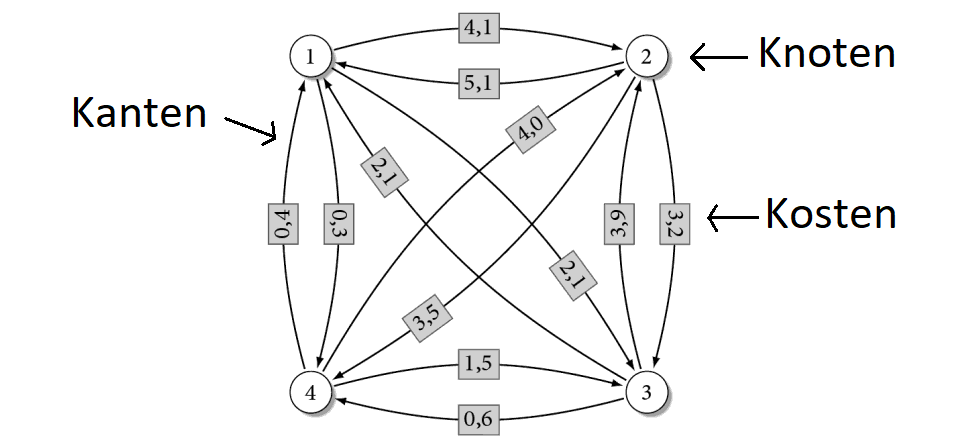
\includegraphics[width=0.9\textwidth]{images/kk_graph_S6.png}
	\caption{Abb. 1.5 von \cite[~S. 6]{Turau:15}. Gewichteter Graph mit Kantenkosten.}
	\label{sec0a}
\end{figure}

\section{Bäume}
Laut \cite{Turau:15} sind Bäume Graphen, die häufig für die Darstellung von hierarchischen Relationen genutzt werden. Ein Baum mit $m$ Knoten hat $m-1$ Kanten.\\
Gegeben ist ein Baum mit Wurzel $w$. Die Tiefe eines Knotens $e$ ist die Anzahl der Kanten von $w$ nach $e$. Die Wurzel $w$ hat die Tiefe 0. Die Höhe des Baumes ist die maximale Tiefe seiner Knoten. Beispiel aus Abb. \ref{sec0b} hat der Baum die Höhe 3 und die Tiefe des Knoten $e$ beträgt 2.
%ist die Höhe des Baumes 3 und die Tiefe des Knotens $e$ ist 2.

\begin{figure} %Von Website
	\centering
	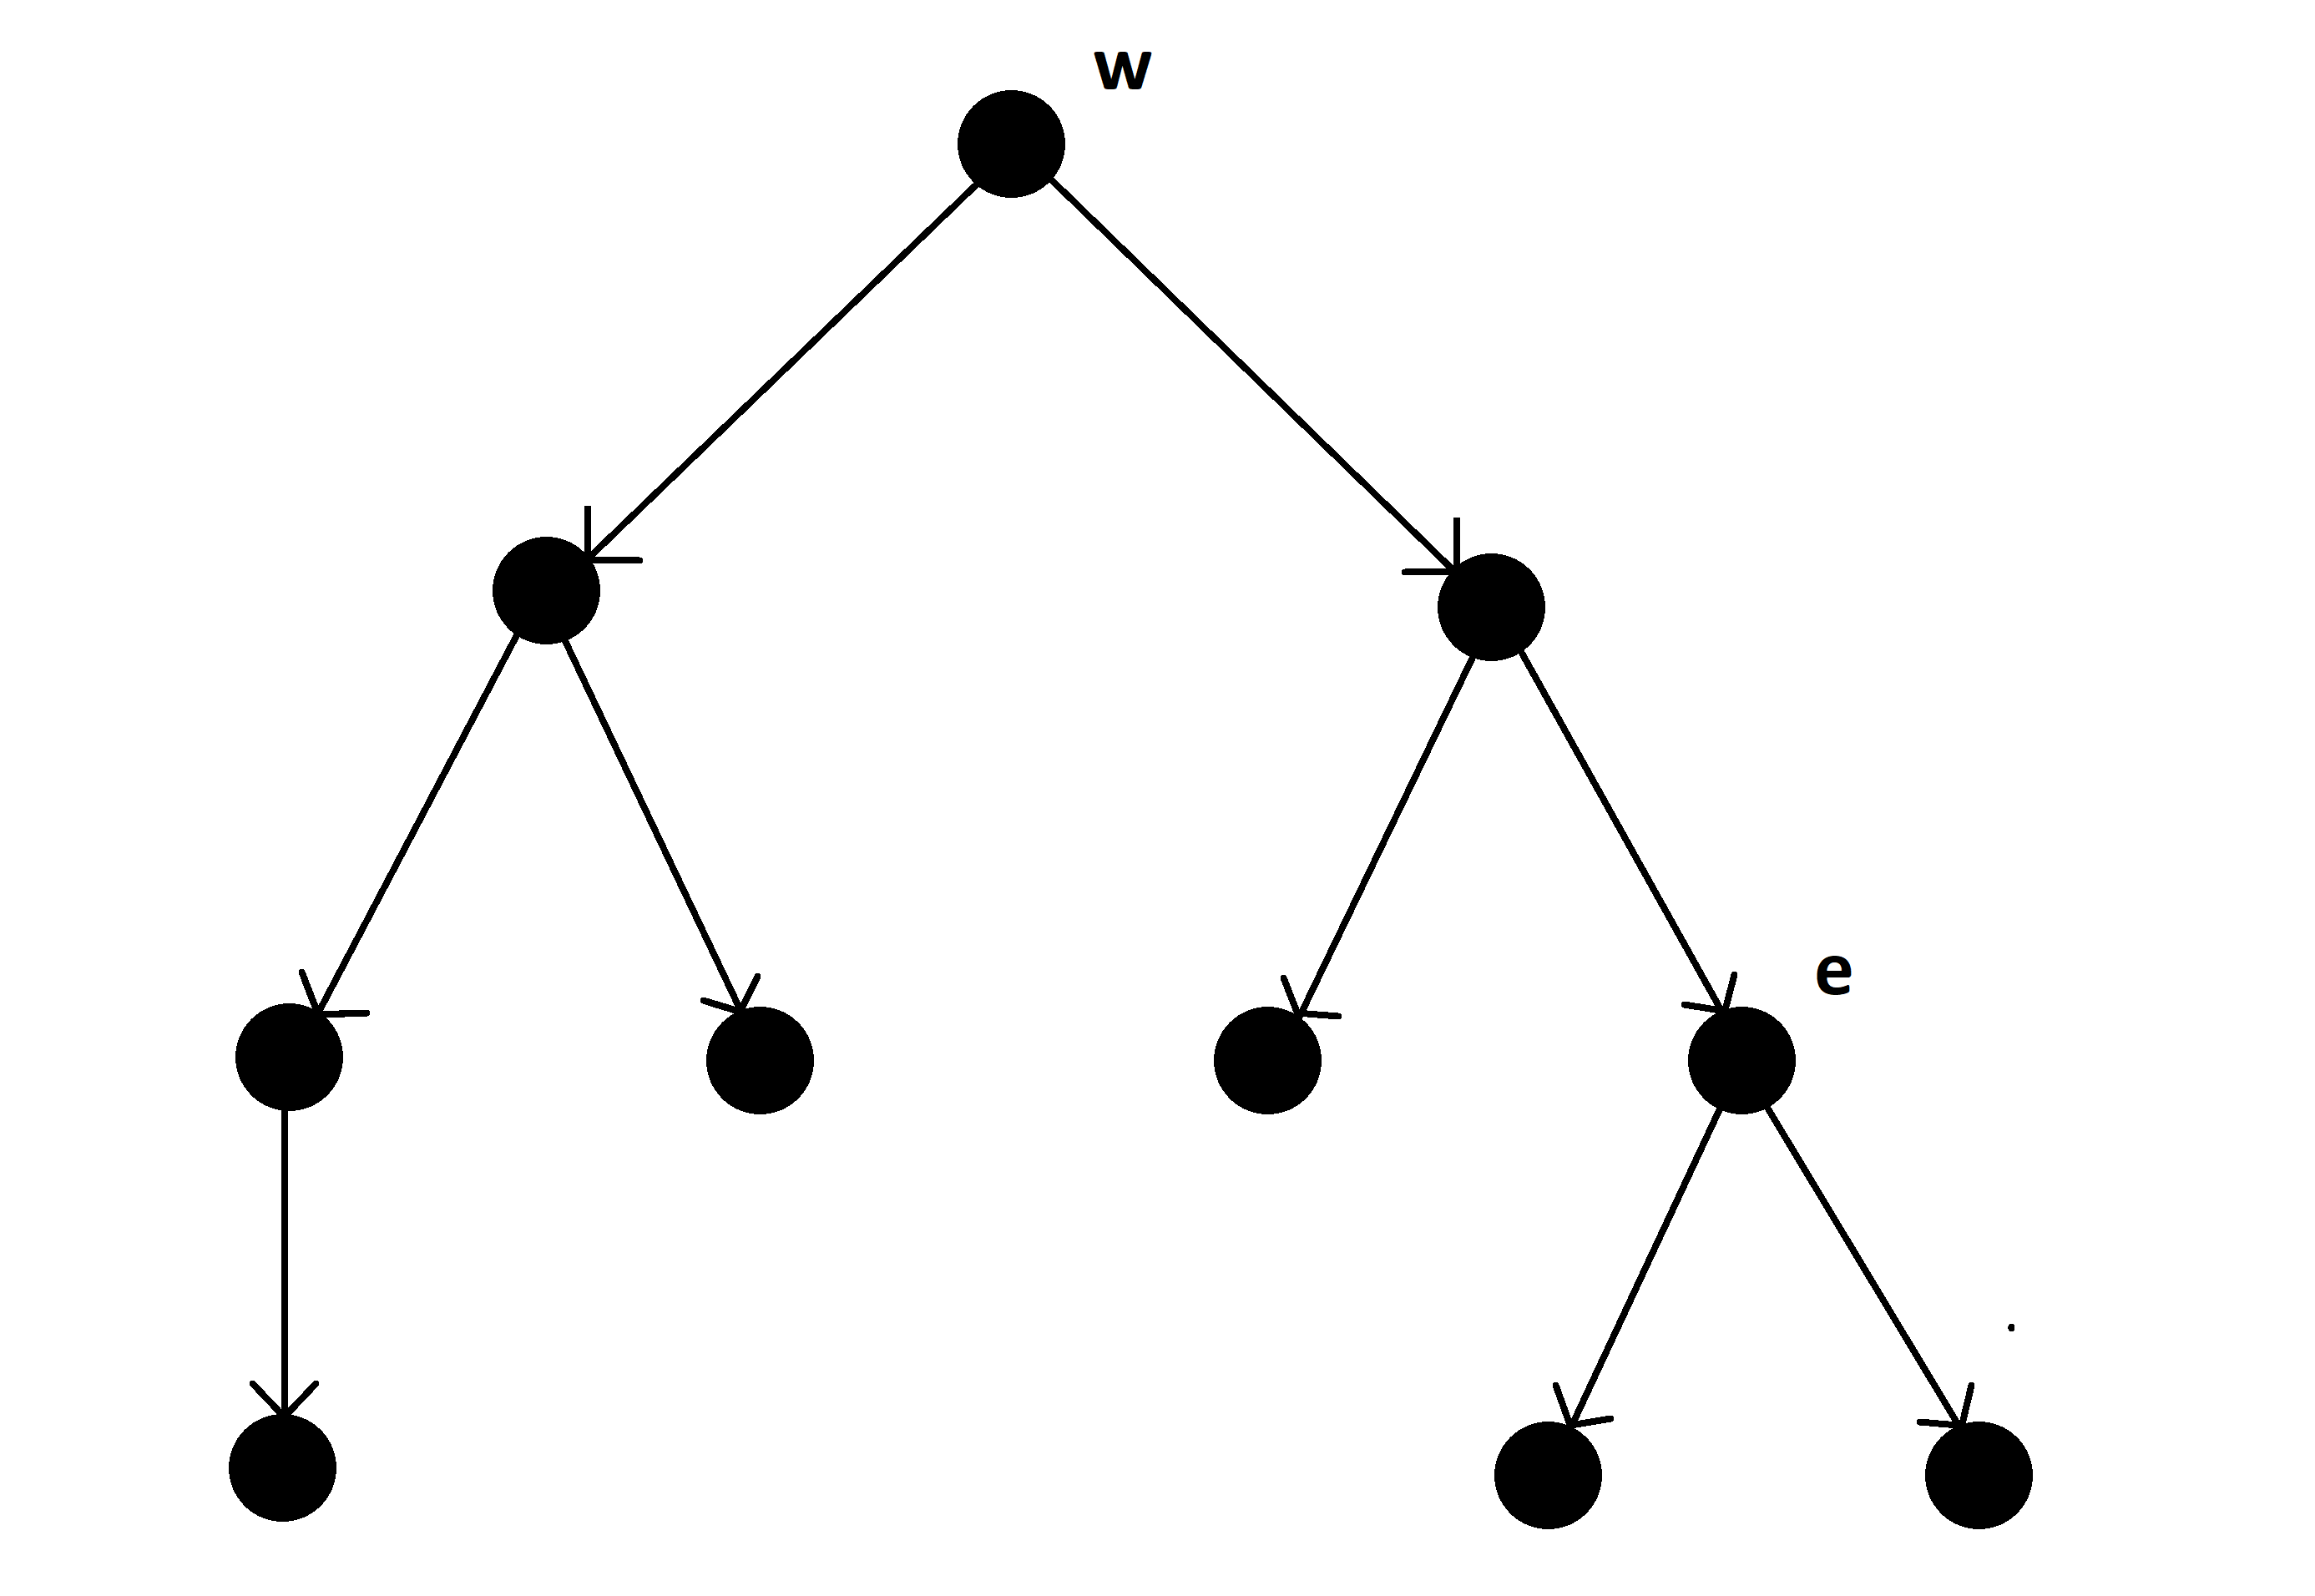
\includegraphics[width=0.5\textwidth]{images/Tree_Graph.png}
	\caption{Ein Baum mit Wurzel \textit{w}}
	\label{sec0b}
\end{figure}

\section{Navigationsnetze (\textit{eng.} Navigation Meshes)}
%\cite{Mesh:11}
%A common strategy for efficiently computing realistic
%paths is to partition the environment into a collection of
%walkable areas. This partition is often referred to as a
%navigation mesh. A useful data structure that can be used to
%construct a navigation mesh is the medial axis. The medial
%axis is the set of all points in an environment that have
%more than one distinct closest point on the boundary of the
%environment
%\cite{Mesh:16}
%(91)
%The behavior of characters may also include crawling, running, and other
%surface-based movement, but we will speak of walking and walkable
%surfaces for simplicity. The walkable surfaces of an environment
%form the free space Efree, which is usually less complex than
%the environment itself.
%A navigation mesh is a representation of Efree as a set of (usually
%polygonal) regions, along with a graph that describes how these
%regions are connected.
%(92)
%Let n be the number of vertices required to define Eobs or Efree
%using simple polygons. We call n the complexity of E.
%(93)
%A walkable environment (WE) is a set of interior-disjoint polygons
%in R3 on which characters can stand and walk. Thus, a WE is a
%clean representation of the free space Efree of a 3DE, based on the
%filtering parameters and character properties mentioned earlier. Any
%two polygons are directly connected if and only if characters can
%walk directly between them.
%
%Now that we have a definition of the free space Efree, we can define
%a navigation mesh as a tupleM= (R; G):
% R = fR0;R1; : : :g is a collection of geometric regions in R3
%that represents Efree. Each region Ri is P-simple, by which
%we mean that a region cannot intersect itself when projected
%onto the ground plane P.
% G = (V;E) is an undirected graph that describes how characters
%can navigate between the regions in R.
%Proper Work
%(91,93) \cite{Mesh:16}
%A Navigation mesh is a representation of the free space as polygonal areas alongside a navigation graph that describes how they are connected. The polygonal areas are the regions where an actor can move, refered to as walkable areas. The navigation graph describes how said actor can move to the next area, as in any surface based movement such as walking. As well as providing the requirements for path planning. pathfinding A navigation mesh can be applied to 3D and 2D environments.
%(91,93)
Nach \cite{Mesh:16} ist ein Navigationsnetz die Darstellung des freien Raums, als polygonale Bereiche. Ein Navigationsgraph definiert die Verbindungen zwischen den Gebieten. Die polygonalen Bereiche sind die Regionen, in denen sich ein Akteur bewegen kann. Sie werden als begehbare Flächen (\textit{eng. walkable areas}) bezeichnet. Der Navigationsgraph beschreibt, wie sich der Akteur in den nächsten Bereichen bewegen kann. Dies tritt bei jeder oberflächen-basierten Bewegung auf, beispielsweise Gehen oder Rennen. Ein Navigationsnetz kann sowohl auf 3D- als auch auf 2D-Umgebungen angewendet werden.

\begin{figure}[H] %Von Website
	\centering
	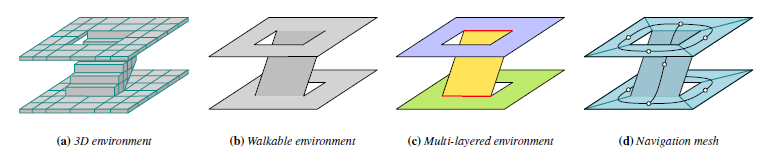
\includegraphics[width=\textwidth]{images/navigation_mesh_16.png}
	\caption{Von \cite[~S. 93]{Mesh:16} \textit{Abb. 2}. Verschiedene Darstellungen einer Umgebung und ein Beispiel für ihr Navigationsnetz. (a) Eine 3D-Umgebung besteht aus unbearbeiteter 3D-Geometrie. (b) Der freie Raum einer 3D-Umgebung. Eine begehbare Umgebung enthält nur begehbare Oberflächen. (c) Eine mehrschichtige Umgebung, ist in Schichten unterteilt. (d) Ein Navigationsnetz ist eine Beschreibung, einer begehbaren Umgebung für Pfadplanungszwecke.}
	\label{sec1a}
\end{figure}
\begin{figure}[H] %Von Website
	\centering
	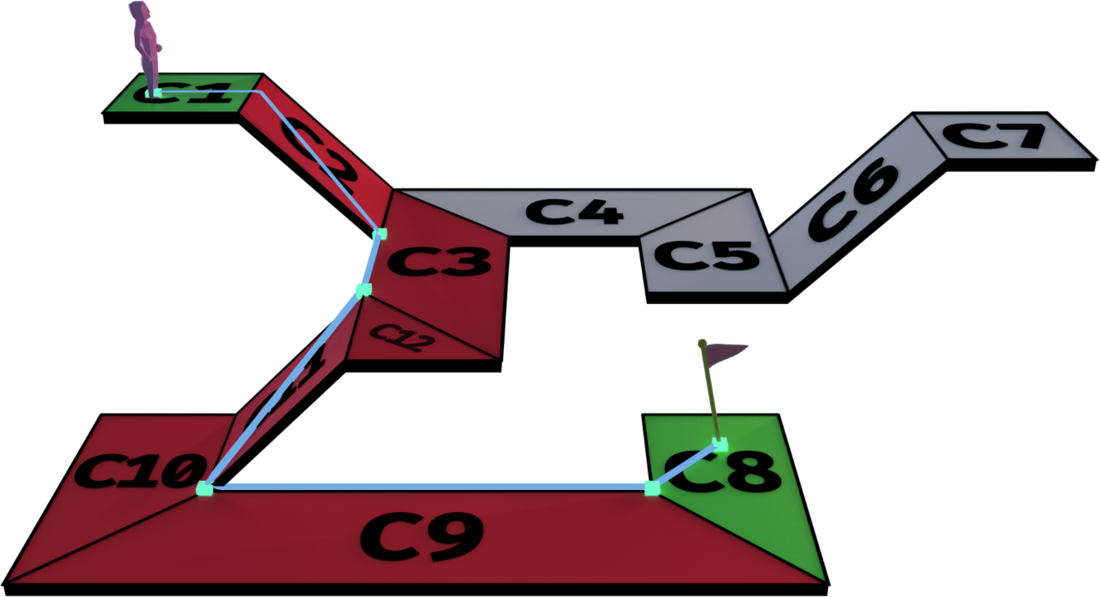
\includegraphics[width=0.6\textwidth]{images/mesh_with_path.png}
	\caption{Von \cite{Mesh:18}: Navigation Mesh mit einem Pfad von Startpunkt C1 bis Endpunkt C8.}
	\label{sec1b}
\end{figure}


\section{Rastergraph (\textit{eng.} Grid Graph)}
%A Star is good for them
%Grids are composed of tiles which lie adjacent to each other
%A raster is put on top of the environment where it will be used. Then a Graph Search with its Tiles is used to find a path in it. For that each Tile possess a travel cost. A common Pathfinding Algorthim used here is A*.
%A common Tile has 4 adjacent Tiles, however more options for a grid are possible. A hextile has six neighbours and the Octile has eight, 4 adjacent like the regular tile and 4 from diagonal movement.
%(1) Raster bestehen aus Kacheln, die nebeneinander liegen.
Raster werden aus einem Netz von zusammenhängenden Kacheln gebildet. Laut \cite{Grid:02} wird ein Raster über die Umgebung gelegt, in der es genutzt werden soll. Wenn die Kacheln als Knoten betrachten werden, kann eine Graphensuche verwendet, um einen Pfad darin zu finden. Dafür besitzt jede Kachel Kanten zu ihren Nachbarn. Ein üblicher Pfadfindungsalgorithmus dafür ist A*.
\\\\
Kacheln können eine verschiedene Anzahl von Nachbarn besitzen. Rechteckigen Kacheln haben vier benachbarte Kacheln. Eine sechseckige Kachel hat sechs Nachbarn. Wenn die Diagonalen betrachtet werden, die normale rechteckige Kachel haben dann acht Nachbarn (siehe Abb. \ref{sec2a}):
%Für den Graph hat eine Kachel typischerweise vier benachbarte Kacheln, es sind jedoch mehr Optionen möglich. Eine sechseckige Kachel hat sechs Nachbarn und die normale rechteckige Kachel hat dann acht, wenn die Diagonalen betrachtet werden (siehe Abb. \ref{sec2a}).
\begin{figure} %Gemacht mit Paint
	\centering
	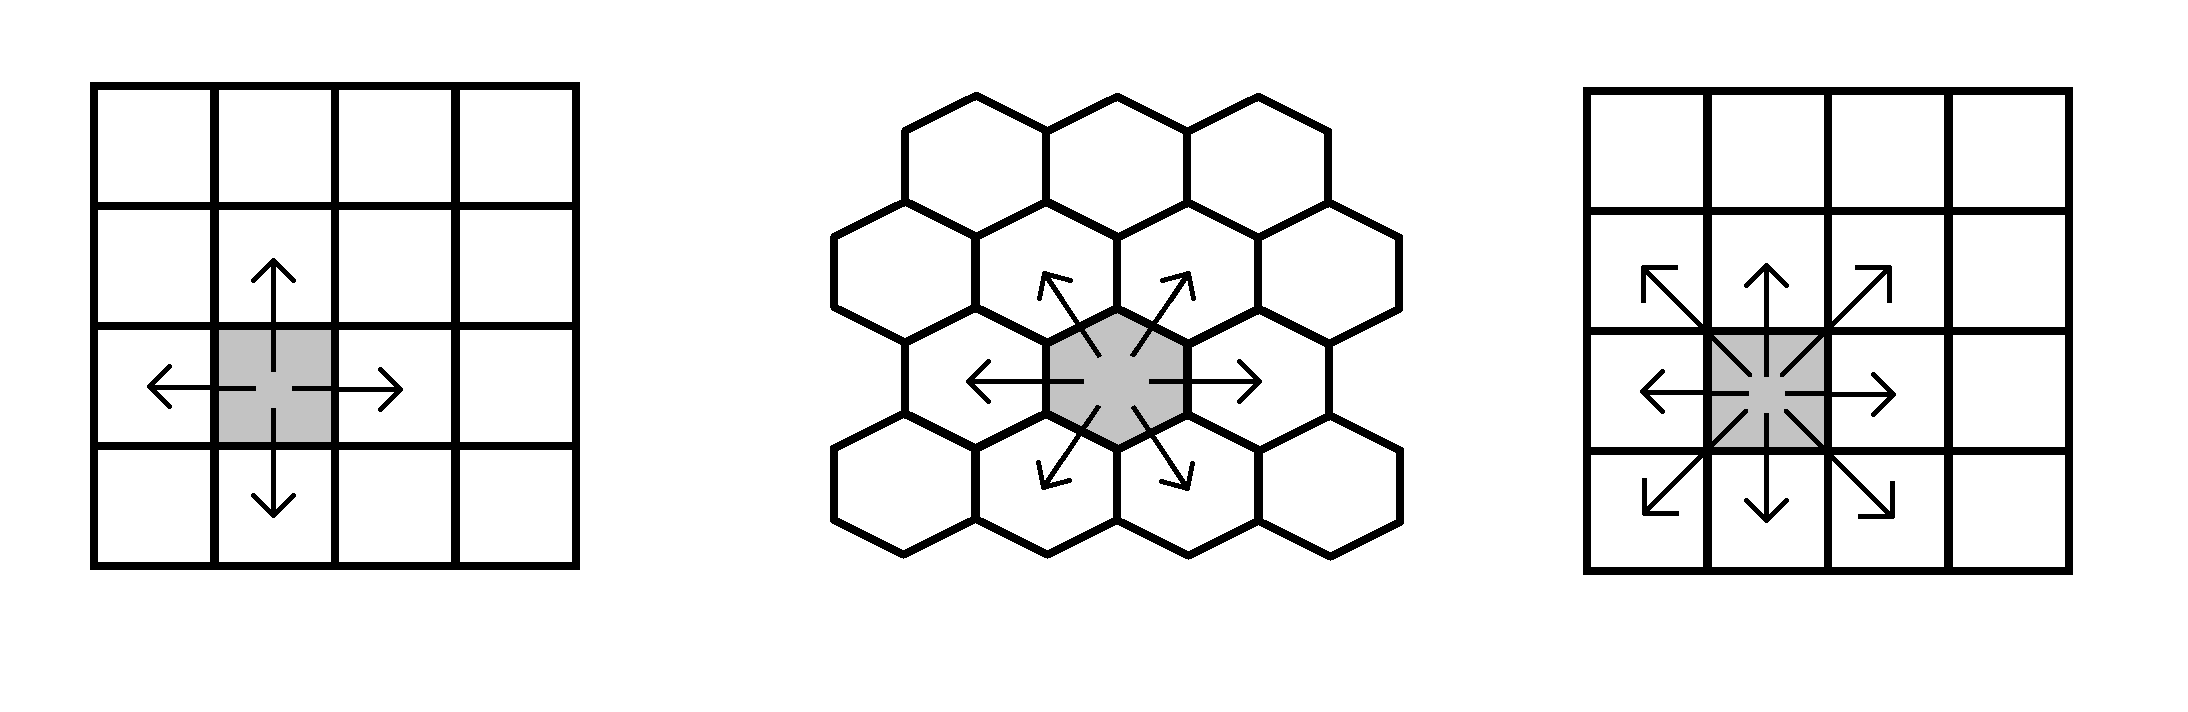
\includegraphics[width=\textwidth]{images/Grid_Tiles.png}
	\caption{Von links nach rechts: Kachel mit 4 Bewegungsoptionen, Hexagon mit 6 Bewegungsoptionen, Kachel mit 8 Bewegungsoptionen.}
	\label{sec2a}
\end{figure}


\section{Sichtbarkeitsgraph (\textit{eng.} Visibility Graph)}
%(110)
%The defining characteristics of a visibility map are that its nodes share an edge if they
%are within line of sight of each other, and that all points in the robot’s free space are
%within line of sight of at least one node on the visibility map.
%
%The standard visibility graph is defined in a two-dimensional polygonal configuration
%space (figure 5.3). The nodes vi of the visibility graph include the start location,
%the goal location, and all the vertices of the configuration space obstacles. The graph
%edges ei j are straight-line segments that connect two line-of-sight nodes vi and vj , i.e.,
%Proper Work
%(110)
%Visibility graphs consist of nodes that share an edge if they are withhin line if sight with each other and no obstacle lies between them. The standard Graph is two dimensional. Possesing the start point, end point and the vertices of the polygons that represent obstacles as nodes.
%
%An example of a visibility graph lies in image ref.
%(110)
%In \cite{Principles:05} ist beschrieben, dass Sichtbarkeitsgraphen aus Knoten bestehen, die in Sichtlinie der Roboter stehen.
In \cite{Principles:05} ist beschrieben, dass aus Knoten, die in Sichtlinie der Roboter stehen, Sichtbarkeitsgraphen gebildet werden. Eine Kante zwischen zwei Punkten gilt nur, wenn keine Hindernisse zwischen ihnen liegen. Der Standardgraph ist zweidimensional. Der Startpunkt und der Endpunkt werden als Knoten dargestellt, sowie die Eckpunkte der Polygone, die Hindernisse darstellen.
\\\\
Ein Beispiel für einen Sichtbarkeitsgraphen findet zeigt Bild \ref{sec3a}.
\begin{figure} %Genommen aus Buch
	\centering
	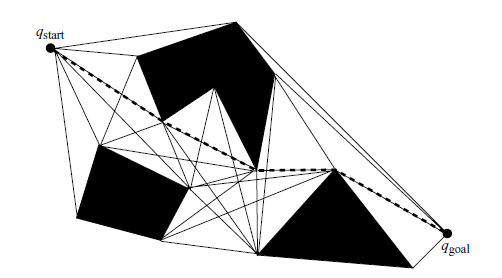
\includegraphics[width=0.8\textwidth]{images/Robot_Motion_Visibility_Graph.png}
	\caption{Von \cite[~S. 111]{Principles:05} \textit{Abb. 5.4} Die Linien begrenzen die Kanten des Sichtbarkeitsgraphen für die drei, als gefüllte Polygone dargestellten Hindernisse. Die gepunktete Linie, stellt den kürzesten Weg zwischen Start und Ziel dar.}
	\label{sec3a}
\end{figure}


%\section{Adjacency graph}
%%bbbb
%
%\section{Punktgraphen (Point Graphs)}
%
%
%\section{(Automatic Navmesh Calculation)}
%
%
%\subsection{Zerteilung des Navmesh (Navmesh Cutting)} 
\chapter{Algorithmen zur Pfadplanung}
\section{Was sind Algorithmen zur Pfadplanung?}
%Es stellt sich die Frage was ein Pfadplanungsalgorithmus "uberhaupt ist, nach [Lavalle] ist es nicht sinnvoll eine genaue Mathematische Definition abzugeben, sondern das Ziel ist eine generelle Idee zu vermitteln und diese mit Beispielen zu veranschaulichen.
%Als eine Antwort zu der Frage wird eine Turing Maschine beschrieben, da damit die meisten Pfadplanungsalgorithmen modelliert werden k"onnen. Turing Maschinen sind "finite-state-machines" welche informationen als String einlesen, diese verarbeiten und aktzeptieren oder ablehnen k"onnen. 
%Mit einer Erweiterung dieses Konzepts kann am Ende auch ein Pfadplan ausgegeben werden. Das Problem bei der Pfadplanung kommt daher, dass die Maschine auf die Umgebung oft reagieren muss, und informationen die durch Sensoren gegeben werden mit einbeziehen m"ussen. 
%Dadurch gibt es keine klare Trennung von der Umwelt und der Maschine solange nicht alle Daten dem System im Vorhinein bekannt sind.[Lavalle]
%\newline
%Ein Ansatzpunkt w"are ein \"on-line algorithmus" der sich aktiv aktualisiert, aber auch dieser kann nicht die gesamte komplexit"at wiederspiegeln. 

Algorithmen zur Pfadplanung sind schwierig mathematisch pr"azise zu definieren. Ein Ansatz ist eine Definition für einen Algorithmus abzugeben und diese anschlie"send zu erweitern, sodass sie den Anspr"uchen der Pfadplanung entspricht. Nach der Church-Turing These ist ein Algorithmus eine Turing Maschine cite{462,891}. Dieser Definition fehlt aber unter anderem, die Repr"asentation der Interaktion eines Roboters mit der Umgebung, wie es in \ref{lav01} dargestellt wird. Daher wird ein Planer \footnote{Planer (engl. planner)} als ein Algorithmus definiert, welcher einen Plan \footnote{Plan (engl. plan)} konstruiert. Der Planer kann sowohl eine Maschine als auch ein Mensch sein und kann dem Konzept einer Turing Maschine entsprechen. Er ist aber nicht darauf limitiert, sondern kann den Anspr"uchen entsprechend erweitert werden.\cite[~S. 19ff]{Lav06} 

\begin{figure} % Hier lieber eine eigene Kombination an Grafiken
	\centering
	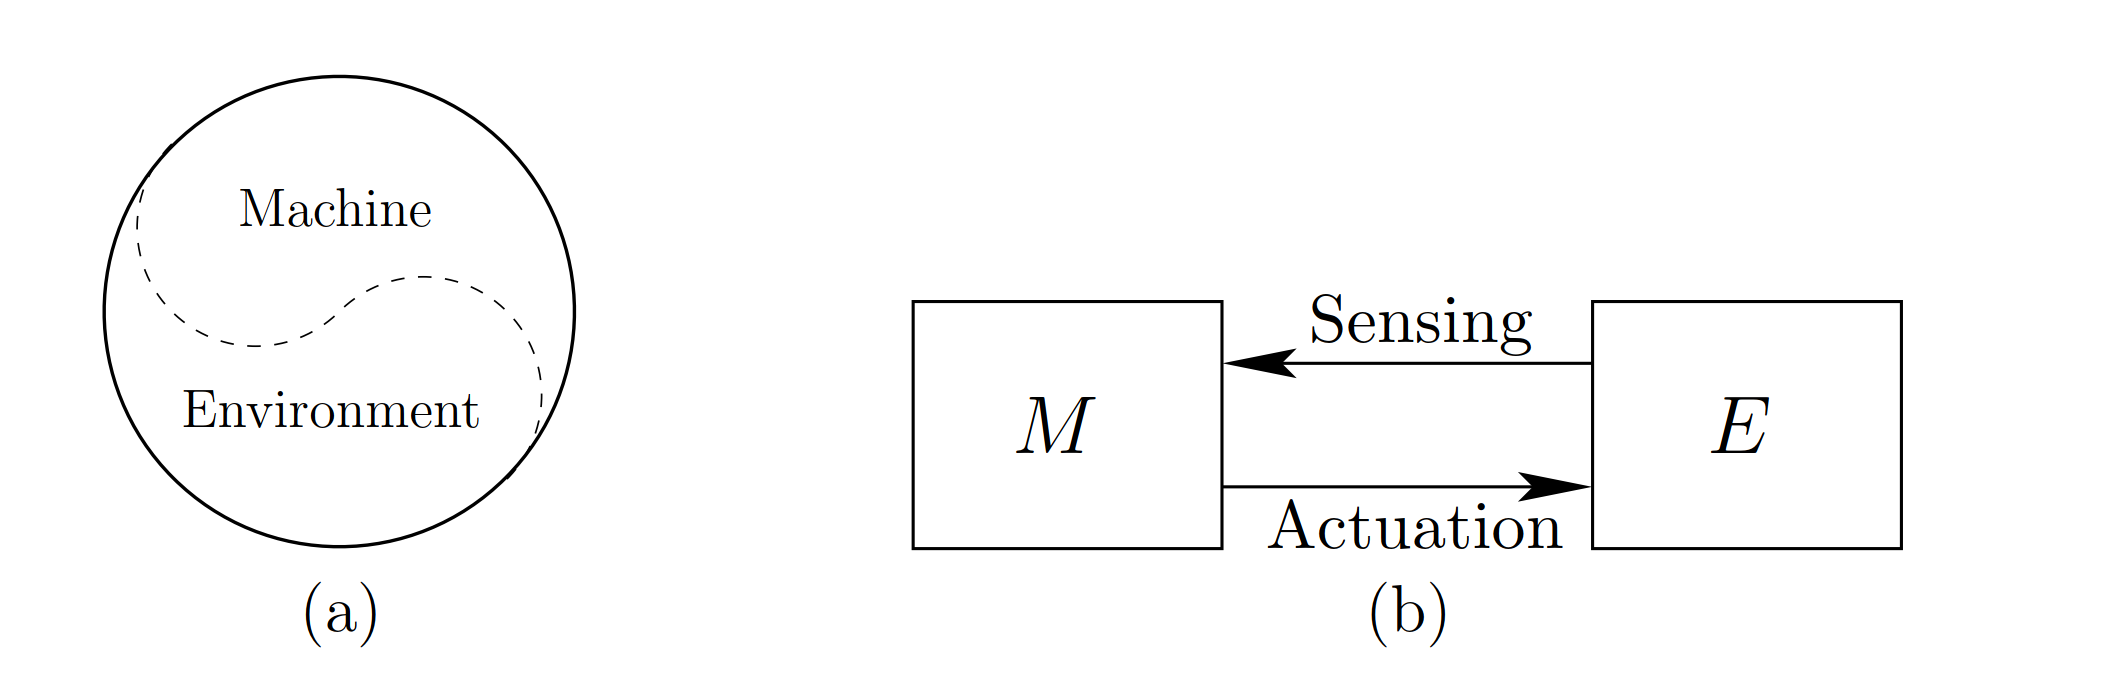
\includegraphics[width=0.6\textwidth]{images/img224.png}
	\caption{Abb. 1.5 von \cite[~S. 20]{Lav06}:  (a) Die Grenze zwischen Maschine und Umgebung ist flie"send, es ist eine Linie die stark in Abh"angigkeit vom Kontext gezogen wird. (b) Ist die Grenze festgelegt, wird angenommen, dass die Maschine M mit der Umgebung U durch Sensorik und den Antrieb interagiert.}
	\label{lav01}
\end{figure}
 



Ein solcher Plan, kann drei unterschiedliche Funktionen erf"ullen. Darunter fallen die Ausf"uhrung \footnote{Ausf"uhrung (engl. Execution)} der Anweisungen in einer Simulation oder durch einen Roboter, die Verbesserung\footnote{Verbesserung (engl. Refinement)} der Eigenschaften in bestimmten Parametern und die hierarchische Einbindung \footnote{Hierarchische Einbindung (engl. Hierarchical Inclusion)} des Plans.
%Ausführung
Pl"ane k"onnen auf zwei weisen ausgef"uhrt werden. Zum einen kann ein Plan als kodierte Eingabe f"ur eine Maschine erstellt werden, welche dadurch programmiert werden kann. Auf diese weise wird die Maschine bei der Ausf"uhrung autonom und kann nicht mehr mit dem Planer interagieren. 
Im zweiten Fall erzeugt der Planer eine Spezialmaschine \footnote{Spezialmaschine (engl. special-purpose machine)}, welche dazu entworfen ist eine Aufgabe zu l"osen.
\newline\\
%Verbesserung
Um einen Plan zu verbessern, wird dieser als Eingabe einem Planer "ubergeben, der daraus einen verbesserten Plan erzeugen soll. 
Anhand von \ref{lav02} wird ersichtlich, wie der gleiche Plan verbessert werden kann, indem verschiedene Aspekte der Problemstellung fokussiert werden.
Die Auswahl der richtigen Kriterien ist schon seit l"angerer Zeit ein Forschungsgebiet in der Robotik, da auch hier Vor- und Nachteile mit verschiedenen Kriterien einhergehen.
\newline\\
%Hierarchische Einbindung
Bei der Hierarchischen Einbindung, wird ein Baum aus Pl"anen erzeugt. Dabei steht an der Wurzel der Hauptplan \footnote{Hauptplan (engl. masterplan)}, welcher andere Pl"ane als Bl"atter in einer Hierarchie einbindet. Ein Plan wird als Aktion betrachtet, die nur als Teil des Gesamtsystem funktioniert. Es wird dadurch erreicht, dass die Abgrenzung zwischen Maschine und Umgebung an verschiedenen stellen gezogen wird.
\newline\cite[~S. 21ff]{Lav06} 

\begin{figure} % Hier lieber eine eigene Kombination an Grafiken
	\centering
	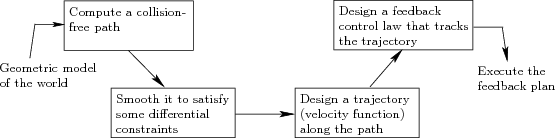
\includegraphics[width=0.6\textwidth]{images/img247.png}
	\caption{Abb. 1.5 von \cite[~S. 20]{Lav06}:  Ein Verbesserungsprozess, der sich in der Robotik bew"ahrt hat.}
	\label{lav02}
\end{figure}

\section{Klassifizierung von Pfadplanungsalgorithmen} % Hier bitte noch ein Bild, das die Unterschiede der einzelnen Klassen sichtbar macht. 
Der Bereich der Pfadplanung ist "au"serst heterogen, da die Umsetzung der Pfadplanung stark von den Vorgaben des Einsatzgebiets abh"angt. 
Es wird Planen in einem diskreten und in einem kontinuierlichen Zustandsraum\footnote{Zustandsraum (engl. state space) Der Zustandsraum beschreibt alle potentiell aufkommenden Zust"ande.} unterschieden. Planen in einem kontinuierlichen Zustandsraum wird Bewegungsplanung genannt, dabei klassifiziert man zwischen Planung mit allen Umgebungsinformationen vorhanden, Planen mit Unsicherheit, sowie Planung mit Bewegungseinschr"ankungen.
Auf die genaue Einteilung der Einsatzgebiete wird in \ref{Kapitel5} noch eingegangen, jedoch ist es f"ur das Verst"andnis der Algorithmen wichtig eine Einsch"atzung der verschiedenen Anforderungen zu erhalten. Im folgenden behandeln wir vor allem die diskrete Pfadplanung, da man daran die Grundlagen erkl"aren kann. \cite[~S. 24ff]{Lav06} 

\section{Diskrete Pfadplanung} \label{Kapitel 4.3} % In diesem Kapitel hätte ich gerne noch ein Bild, das das Konzept der diskreten Pfadplanung auf einen Blick veranschaulicht veranschaulicht

Diskrete Pfadplanung dient in der meisten Literatur als Einstiegspunkt. Das kommt daher, da der state space entweder endlich oder z"ahlbar unendlich ist.\\
Au"serdem müssen dadurch keine geometrischen Modelle oder Bewegungseinschr"ankungen \footnote{Bewegungseinschr"ankungen (engl. differential constraints)} im Entwurf des Algorithmus beachtet werden.
% Der Planer weis über alles bescheit, die struktur ist regelmaeßig
Je nach Anforderung werden die drei Teilgebiete feasible planning \footnote{feasible planning (Dt. durchführbares Planen) im folgenden FP}, optimales planen und logik basierte repr"asentation unterschieden. Die vorherrschenden Algorithmen in diesem Bereich, sind der Dijkstra Algorithmus aus der Graphentheorie und der daraus abgeleitete A*-Algorithmus. Von diesem gibt es noch eine Reihe weiterer Abwandlungen, die alle eine Optimierung auf ein bestimmtes Einsatzgebiet zum Ziel haben.\cite[~S. 27]{Lav06} \\
Wie man diese Optimierung durchführen kann wird im folgenden an verschiedenen Algorithmen erl"autert. Optimales Planen unterscheidet sich nur insofern vom feasible planning, als das der gefundene Pfad in verschiedenen Kriterien wie Zeit, Distanz oder auch der Anzahl an Drehungen eines Roboters optimiert werden kann.\cite[~S. 43]{Lav06} \\
Der state space spielt in der Pfadplanung eine zentrale Rolle, dabei kann zwischen Zust"anden durch die Ausf"uhrung von Aktionen gewechselt werden. Die verf"ugbaren Aktionen werden in einem Aktiosraum\footnote{Aktionsraum (engl. action space) } zusammengefasst, au"serdem ist als Teil des Planungsproblem ein Satz von Zielzust"anden\footnote{Zielzust"ande (engl. goal states)} definiert. 
Da ein Zustandsgraph schnell sehr gro"s werden kann wird dieser meist nicht komplett "ubergebe, sondern diese wird im Laufe des Planungsprozess aufgedeckt.
\cite[~S. 43]{Lav06} \\
Wie man effektiv durch den Zustandsraum navigiert um einen goal state zu erreichen ist das Thema des folgenden Absatz.
\begin{figure}
\centering
\subsection*{Formulierung 4.3 (Discrete Feasible Planning)}
\begin{enumerate}
	\item Ein nichtleerer Zustandsraum $X$, der endlich viele oder z"ahlbar unendlich viele Zust"ande beschreibt.  
	\item F"ur jeden Zustand $x \in X$ , ein endlicher Aktionsraum $U( \, x) \,$.
	\item Eine Zustands"ubergangsfunktion $f$ welche einen Zustand  $f( \, x,u) \, \in X$ für jedes $x \in X$  und $u \in U( \, x) \,$ erzeugt. Die Zustands"ubergangsgleichung ist von $f$ als $x' = f( \, x,u )\, $ abgeleitet.
	\item Ein Anfangszustand $ x_{I} \in X$.
	\item Ein Satz mit Zielzust"anden $X_{G} \subset X$.
\end{enumerate}
\caption{In Anlehnung an Formulation 2.1 von \cite[~S. 29]{Lav06}}
\label{lav02}
\end{figure}
%1. A nonempty state space X, which is a finite or countably infinite set of states.
%2. For each state x ∈ X, a finite action space U(x).
%3. A state transition function f that produces a state f(x, u) ∈ X for every
%x ∈ X and u ∈ U(x). The state transition equation is derived from f as
%x′ = f(x, u).
%4. An initial state xI ∈ X.
%5. A goal set XG ⊂ X.

\subsection {Feasible Planning} % Hier sollte mit einem Code Beispiel ein allgemeingültiger algorithmus veranschaulicht werden. Darauf kann dann später wieder eingegangen werden und veränderungen im code können mit veränderungen in der Funktionalität in kontakt gesetzt werden.
Ein allgemeiner Beispielalgorithmus ist in [Lavalle] gegeben. Als Beispiel f"ur diskrete Pfadplanung kann die Bewegung auf einem endlichen 2D Netz mit Hindernissen gesehen werden. 
Dieses hat einen Startpunkt und einen Zielpunkt und muss einen Pfad zwischen diesen Punkten finden. Bei der Feasible Planning ist es ausreichend einen funktionierenden Pfad zu finden und es wird noch nicht darauf geachtet ob dieser optimal in Hinblick auf L"ange ist.
\newline
Die Algorithmen die hier verwendet werden sind Algorithmen zur Graphensuche die das Problem aus einer Planungsperspektive angehen. Es ist wichtig, dass diese Algorithmen systematisch sind. Das bedeutet, dass bei einem endlichen Graphen alle zust"ande besucht werden, au"serdem muss beachtet werden welche Zust"ande schon besucht wurden. Bei einem unendlichen Graphen ist die Definition insofern anders ist, dass es ausreicht, dass der Algorithmus zu einer L"osung bei l"osbaren Problemen kommt. 
\newline 
Eine generelle Template f"ur einen Suchalgorithmus kann durch drei Zust"ande repr"asentiert werden. 
Ein unentdecktes Feld wurde noch nicht besucht und ist daher auch noch nicht bekannt. Ein Totes Feld kann nichts mehr zur Suche Beitragen, da schon die angrenzenden Felder entdeckt wurden. Felder die noch am Leben sind haben noch potentielle Nachbarfelder die am leben sind.  
\newline
Der einzige wirkliche Unterschied zwischen Planungsalgorithmen kommt durch die Auswahl eines Sortieralgorithmus f"ur die Priority Queue in welcher die n"achsten abzuarbeitenden Elemente enthalten sind. Die einfachsten Varianten sind hier FIFO(First-In First-Out), hier wird immer das Element gew"ahlt das am l"angsten gewartet hat. Dadurch entsteht eine kreisf"ormig expandierende Suche. 
\newline
Damit der gefundene Weg vom Start zum Ziel rekonstruiert werden kann muss jeder Knoten seinen Vorg"angerknoten abspeichern. Das erm"oglicht es den Weg sp"ater zur"uckzuverfolgen. 
\newline
Um darzustellen welchen einfluss die Sortierfunktion auf das Verhalten der Algorithmus hat werden im folgenden einige Algorithmen pr"asentiert.
Diese sind alle eine Abwandlung des Algorithmus aus der Abbildung. 
\newline
\newline
\subsubsection{Breath-first search} Breadth first search verwendet die oben angesprochene FIFO Warteschlange wodurch sich eine kreisf"ormige expansion ergibt, die auch die vorraussetzung f"ur systematische Algorithmen erf"ullt. Bei diesem algorithmus k"onnen einige kontrollmechanismen eingespart werden die sonst zur kontrolle der Expanionn"otig werden, jedoch verschwendet dieser Algorithmus durch die gleichm"assige ausbreitung relativ viele Zyklen. 
\newline
\newline
\subsubsection{Depth first search} Depth first search verwendet einen Stack als warteschlange, das heisst LIFO(Last-In First-Out) dies erzeugt eine aggresive Expansion in eine bestimmte Richtung.
Da die Richtung in die am anfang zum expandieren gew"ahlt wird zuf"allig ist, ist diese Methode nicht wirklich zielf"uhrend, da sie nur bei endlich vielen Knoten systematisch ist. 
\subsubsection{Djikstra Algorithmus}
Der Djiksta Algorithmus findet einen optimalen Pfad kann aber auch feasible pfade finden. Der Unterschied zu den vorhergehenden Algorithmen ist das hier Aktionen mit einander verglichen werden um die die mit den besseren Chancen ein gutes ergebnis zu finden erst auszuf"uhren. Das vorgehen von Dijkstra ist weitgehend bekannt und kann bei [Lavalle] nachgelesen werden.

\subsubsection{A-Stern} 
Der A* Suchalgorithmus ist eine Erweiterung von Dijkstra's Algorithmus und mit dem Ziel, die Anzahl der gesamtschritte zu minimieren,
indem eine Heuristik eingef"uhrt wird die die Suche in die Richtung des Ziels f"uhrt. Dabei k"onnen unterschiedliche Werte f"ur die Heuristik gew"ahlt werden,
jedoch wird meistens die der direkte Abstand zwischen dem Start und dem Endpunkt als Wert genommen. Das daraus entstehende verhalten zeichnet sich dadurch aus dass der Algorithmus solange in die Richtun des Ziels sucht, bis er auf ein hindernis st"o"st und erst dann versucht dieses Hindernis zu umgehen.
\newline
TODO Mehr informationen
\subsubsection{weitere}
Weitere Abwandlungen sind Best first search, hier wird die Warteschlange nach einer erwarteten \"cost-to-go" sortiert. 
Desweiteren gibt es noch abwandlungen wie Interative Deepening das den Depth first Algorithmus in abgewandelter form einsetzt. 
R"uckw"artssuche und Bidirektionale suche verhalten sich so wie ihr es beschreibt und kommen alle mit eigenheiten. 


%Simon fährt fort
\section{Planung mit kontinuierlichem Zustandsraum}
Lorem ipsum dolor sit amet, consetetur sadipscing elitr, sed diam nonumy eirmod tempor invidunt ut labore et dolore magna aliquyam erat, sed diam voluptua. At vero eos et accusam et justo duo dolores et ea rebum. Stet clita kasd gubergren, no sea takimata sanctus est Lorem ipsum dolor sit amet. Lorem ipsum dolor sit amet, consetetur sadipscing elitr, sed diam nonumy eirmod tempor invidunt ut labore et dolore magna aliquyam erat, sed diam voluptua. At vero eos et accusam et justo duo dolores et ea rebum. Stet clita kasd gubergren, no sea takimata sanctus est Lorem ipsum dolor sit amet.

 
%%oder einer Grafik die ich noch schreiben muss. 
%\section{Bewegungsplanung}
%% Die Planung muss zus"atzlich noch die Bewegung in der Umgebung in betracht ziehen. 
%\subsection{Sampling-Based Motion Planning}
%\subsection{Combinatorial Motion Planning}
%\section{Planen mit Unsicherheit}
%% Hier kommt noch unsicherheit in der Umgebung hinzu, also auch dynamische Systeme
%\subsection{Entscheidungstheorie}
%\subsection{Planen mit Unsicherheiten in der Sensorik}
%\section{Planen mit Differentialen Einschr"ankungen}
%% Hier müssen bewegungseinschr"ankungen die durch den Verwendeten Roboter einhergehen beachtet werden. 
%\subsection{Sampling-Based Planning under Differential Constraints}


\chapter{Zusammenfassung und Ausblick}

In diesem Kapitel soll die Arbeit noch einmal kurz zusammengefasst werden. Insbesondere sollen die wesentlichen Ergebnisse Ihrer Arbeit herausgehoben werden. Erfahrungen, die z.B. Benutzer mit der Mensch-Maschine-Schnittstelle gemacht haben oder Ergebnisse von Leistungsmessungen sollen an dieser Stelle pr�sentiert werden. Sie k�nnen in diesem Kapitel auch die Ergebnisse oder das Arbeitsumfeld Ihrer Arbeit kritisch bewerten. W�nschenswerte Erweiterungen sollen als Hinweise auf weiterf�hrende Arbeiten erw�hnt werden.
% ...
%--------------------------------------------------------------------------
\backmatter                        		% Anhang
%-------------------------------------------------------------------------
\bibliographystyle{geralpha}			% Literaturverzeichnis
\bibliography{literatur}     			% BibTeX-File literatur.bib
%--------------------------------------------------------------------------
\printindex 							% Index (optional)
%--------------------------------------------------------------------------
\begin{appendix}						% Anh�nge sind i.d.R. optional
   \chapter{Glossar}

%\abbreviation{DisASTer}		{DisASTer (Distributed Algorithms Simulation Terrain), A platform for the Implementation of Distributed Algorithms}
%\abbreviation{DSM}			{Distributed Shared Memory}
%\abbreviation{AC}			{Linearisierbarkeit (atomic consistency)}
%\abbreviation{SC}			{Sequentielle Konsistenz (sequential consistency)}
%\abbreviation{WC}			{Schwache Konsistenz (weak consistency)}
%\abbreviation{RC}			{Freigabekonsistenz (release consistency)}
			% Glossar   
\end{appendix}

\end{document}
